%\documentclass[jou]{apa6}
\documentclass[11pt]{article}
\usepackage{ucs}
\usepackage[utf8x]{inputenc}
\usepackage{changepage}
\usepackage{graphicx}
\usepackage{amsmath}
\usepackage{gensymb}
\usepackage{amssymb}
\usepackage{enumerate}
\usepackage{tabularx}
\usepackage{lipsum}
\usepackage{hyperref}
\usepackage{fancyvrb}

\oddsidemargin 0.0in
\evensidemargin 0.0in
\textwidth 6.27in
\headheight 1.0in
\topmargin -0.1in
\headheight 0.0in
\headsep 0.0in
\textheight 9.0in

\usepackage{xcolor}

\setlength\parindent{0pt}

\newenvironment{myenv}{\begin{adjustwidth}{0.4in}{0.4in}}{\end{adjustwidth}}
\renewcommand{\abstractname}{Anotācija}
\renewcommand\refname{Atsauces}



\newcounter{alphnum}
\newenvironment{alphlist}{\begin{list}{(\Alph{alphnum})}{\usecounter{alphnum}\setlength{\leftmargin}{2.5em}} \rm}{\end{list}}


%16.3-6

\makeatletter
\let\saved@bibitem\@bibitem
\makeatother

\usepackage{bibentry}



\begin{document}
\thispagestyle{empty}


\begin{center}
{\Large C++ Exercise 5: Circularly Linked Lists}
\end{center}

%\begin{abstract}
%This exercise shows how to implement a circularly linked list 
%of integers. 
%% https://softwareengineering.stackexchange.com/questions/149555/difference-between-immutable-and-const
%% Our rational numbers are "immutable"
%\end{abstract}


{\bf Deadline:} Monday, October 12, 2020 by 23:59:59 EEST Timezone.\\ 
{\bf How to submit:} Check your code into your GitHub repository, the default {\tt master} branch, 
tag it as {\tt ex05submit} (all lowercase, no dashes).\\
{\bf Grading:} This exercise is worth 30\textperthousand (or $3\%$) of the total grade.


\vspace{10pt}
Develop a software that receives a list of integers
and adds them to a circular linked list (implemented 
as pointers). See Section 3.4.1 in the textbook. 

\vspace{10pt}
{\bf Input}

The first line contains number $N$ (the number of integers to add
into the initial circularly linked list). 
After that the input contains exactly $N$ integers 
(not necessarily different) that fit into the {\tt int} data type.
All these integers are written on a single line.  
After that there are one or more operations that insert or delete 
things at certain places in the circularly linked list 
(we assume that the cursor does not change once the circularly 
linked list becomes nonempty).


\vspace{10pt}
{\bf Output}

The output is a list of integers (starting from the 
circularly linked list's ``front'' element - pointed to by the cursor) 
after all the insert and delete
operations performed. 



\vspace{10pt}
{\bf Implementation Details}

\begin{enumerate}
\item Implement files {\tt CircleList.cpp} (and {\tt CircleList.h})
that ensure circularly linked list of integers. 
Also implement {\tt CircleListMain.cpp} to read input and write to 
output. 
\item If you need any other C++ classes or structures (for a single 
Circularly Linked List node, custom exception {\tt OutOfBoundsException}
etc.) add these structures to 
your {\tt CircleList.cpp} and {\tt CircleList.h} respectively. 
We do not test any of them separately. 
\item Implement the functions of a circularly linked list to support 
the ADT of this abstract data structure (see Figure~\ref{fig:ex05-circularly-linked-lists}).
\item Even if you do not need some of the functions (for insertion or 
deletion), make sure that they are still implemented - as we might use them 
in the next lab that will be continued next week. 
\item Ensure that your code has destructors for all the data 
structures you dynamically create and that your code has no memory leaks.
\item If the command cannot be performed (insert or delete 
position is larger than the current size of the circularly linked list), 
thrown a custom exception {\tt OutOfBoundsException}.
\end{enumerate}

\begin{figure}[!htb]
\center{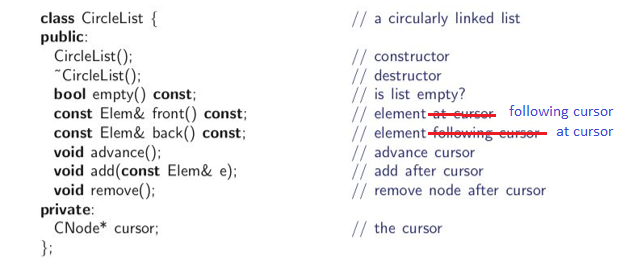
\includegraphics[width=5in]{ex05-circularly-linked-lists.png}}
\caption{\label{fig:ex05-circularly-linked-lists} Circularly linked lists.}
\end{figure}


\vspace{10pt}
\begin{tabular}{@{}ll@{}}
\begin{minipage}[t]{0.49\columnwidth}
Sample input {\bf test01in.txt}:
\begin{verbatim}
6
11 12 13 14 15 16
INS 2 1000
\end{verbatim}
\end{minipage} 
&
\begin{minipage}[t]{0.49\columnwidth}
Expected output {\bf test01expected.txt}:
\begin{verbatim}
11 12 1000 13 14 15 16
\end{verbatim}
\end{minipage} 
\end{tabular}



\vspace{10pt}
\begin{tabular}{@{}ll@{}}
\begin{minipage}[t]{0.49\columnwidth}
Sample input {\bf test02in.txt}:
\begin{verbatim}
6
11 12 13 14 15 16
DEL 2
\end{verbatim}
\end{minipage} 
&
\begin{minipage}[t]{0.49\columnwidth}
Expected output {\bf test02expected.txt}:
\begin{verbatim}
11 12 14 15 16
\end{verbatim}
\end{minipage} 
\end{tabular}



\vspace{10pt}
\begin{tabular}{@{}ll@{}}
\begin{minipage}[t]{0.49\columnwidth}
Sample input {\bf test03in.txt}:
\begin{verbatim}
6
11 12 13 14 15 16
INS 0 100
DEL 2
\end{verbatim}
\end{minipage} 
&
\begin{minipage}[t]{0.49\columnwidth}
Expected output {\bf test03expected.txt}:
\begin{verbatim}
100 11 13 14 15 16
\end{verbatim}
\end{minipage} 
\end{tabular}




\vspace{10pt}
\begin{tabular}{@{}ll@{}}
\begin{minipage}[t]{0.49\columnwidth}
Sample input {\bf test04in.txt}:
\begin{verbatim}
6
11 12 13 14 15 16
DEL 6
\end{verbatim}
\end{minipage} 
&
\begin{minipage}[t]{0.49\columnwidth}
Expected output {\bf test04expected.txt}:
\begin{verbatim}
OutOfBoundsException
\end{verbatim}
\end{minipage} 
\end{tabular}


\vspace{10pt}
\begin{tabular}{@{}ll@{}}
\begin{minipage}[t]{0.49\columnwidth}
Sample input {\bf test05in.txt}:
\begin{verbatim}
6
11 12 13 14 15 16
INS 6 101
\end{verbatim}
\end{minipage} 
&
\begin{minipage}[t]{0.49\columnwidth}
Expected output {\bf test05expected.txt}:
\begin{verbatim}
11 12 13 14 15 16 101
\end{verbatim}
\end{minipage} 
\end{tabular}


\vspace{10pt}
\begin{tabular}{@{}ll@{}}
\begin{minipage}[t]{0.49\columnwidth}
Sample input {\bf test06in.txt}:
\begin{verbatim}
6
11 12 13 14 15 16
INS 7 101
\end{verbatim}
\end{minipage} 
&
\begin{minipage}[t]{0.49\columnwidth}
Expected output {\bf test06expected.txt}:
\begin{verbatim}
OutOfBoundsException
\end{verbatim}
\end{minipage} 
\end{tabular}






\vspace{10pt}
{\bf Running Unit tests (Check2)}

Inserting and deleting items from lists of integers 
can be implemented in many ways. 
The operations that we want 
(INS and DEL at certain positions in the list) can be 
easily expressed using the circularly linked list ADT
(Figure~\ref{fig:ex05-circularly-linked-lists}). 

To distinguish ``high-level mistakes'' in our code
(e.g. handling input/output incorrectly or misinterpreting where
we need to insert and delete) from ``low-level mistakes'' 
(wrongly implemented data structure), we suggest 
that you run Unit tests on {\tt CircleList} classes

In fact, out of 30 points for this exercise, 10 points will be
given for satisfying the unit tests. 
A few notes before you apply the {\tt CircleList} class to 
the EX05 problem (inserting/deleting integers at certain positions): 

\begin{enumerate}
\item The function {\tt front()} returns integer value following the
cursor, but {\tt back()} returns the integer value currently under
the cursor. (This is explained in the textbook too, just the two comments 
have switched places on p.130). 
\item In order to throw {\tt OutOfBoundsException} whenever we 
insert at position that does not currently exist (and also is not next
to one that currently exists), we need to know the current size 
of the circularly linked list. Therefore the {\tt getSize()} method
in the UML diagram (Figure~\ref{fig:ex05-uml-diagram}). 
The same function is needed as we delete from that list.
%(Size is easy to maintain: You can initialize it to $0$ as you create 
%an empty list, then increment it every time you call {\tt add()}, and
%decrement every time you call {\tt remove()}.)
\item Adding and removing elements only happen next to the head/cursor. 
If you need to add/remove in any other place, you need to call 
{\tt advance()} certain number of times. 
And after the operation you need to return the list to the original 
cursor position. It can be achieved in two ways: Either you call {\tt 
advance()} many times to run around the whole list. 
Or you can also implement {\tt retreat()} that works in the opposite
direction than {\tt advance()} (head travels back using {\tt prev} pointer
in {\tt CNote}.)
\end{enumerate}

Our Unit tests are implemented using Catch2 framework; 
see \url{https://github.com/catchorg/Catch2}. 
It means that you download {\tt catch.hpp} and place
it in your project directory. Tests are
organized into testcases and sections. 
Each of testcases (or sections therein) can 
call your {\tt CircleList} implementation.

Since this file ({\tt Catch2TestRunner.cpp}) creates its
own {\tt main()} method, you cannot run it in the same executable
as the one created by the {\tt CircleListMain.cpp}. 
Please refer to the {\tt Makefile} and the testcases
{\tt Catch2TestRunner.cpp} for details - under {\bf EX05} 
lab section in\\
\url{http://linen-tracer-682.appspot.com/data-structures/assignments.html}.




\begin{figure}[!htb]
\center{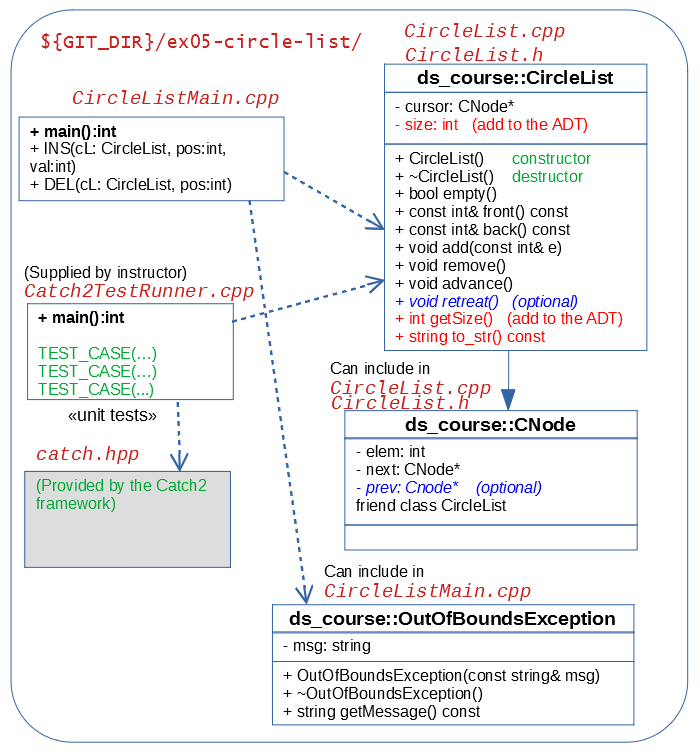
\includegraphics[width=5in]{ex05-uml-diagram.png}}
\caption{\label{fig:ex05-uml-diagram} Classes for EX05.}
\end{figure}



%% 
%% Sth.
%% 


%% External demo... 
%% Homogeneous coordinates in 2D - an example that paints SVG. 
%% It should be able to eat some transformation matrices, apply multiplication
%% Then it takes some figure (e.g. L-shape) - and arranges it somehow.


%% Some discussion why rational numbers should be made immutable (note that the 
%% https://introcs.cs.princeton.edu/java/92symbolic/Rational.java.html

%% https://en.wikipedia.org/wiki/Rep-tile
%% 

%% https://scicomp.stackexchange.com/questions/4666/what-is-the-criteria-for-switching-between-strassens-and-regular-matrix-multipl

%% https://github.com/saif86/Rational-Numbers---Operator-Overloading/blob/master/RationalNumber.h
%% https://github.com/saif86/Rational-Numbers---Operator-Overloading/blob/master/RationalNumber.cpp

\end{document}



\vspace{10pt}
{\bf Continuation of this exercise for the next week}

\begin{enumerate}
\item Implement the \textit{circular linked list}, an abstract data type where:
\begin{itemize}
\item each node contains its value and a link to the next node
\item the link on the last node points back to the first node.
\end{itemize}
\vspace{10pt}
\[
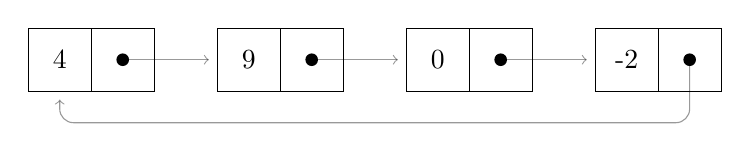
\begin{tikzpicture}[scale=.8,link/.style={opacity=.4,->,shorten >=3pt}]
\draw (0,0) rectangle (2,1); \draw (1,0)--(1,1);
\draw (3,0) rectangle (5,1); \draw (4,0)--(4,1);
\draw (6,0) rectangle (8,1); \draw (7,0)--(7,1);
\draw (9,0) rectangle (11,1); \draw (10,0)--(10,1);
\foreach \x\n in {0/4, 1/9, 2/0, 3/-2}{
  \node at (3*\x+.5,.5) {\n};
  \fill[black] (3*\x+1.5,.5) circle (.1);
}
\draw[link] (1.5,.5)--(3,.5);
\draw[link] (4.5,.5)--(6,.5);
\draw[link] (7.5,.5)--(9,.5);
\draw[link,rounded corners=5pt] (10.5,.5)--++(270:1)--++(180:10)--++(90:.5);
\end{tikzpicture}
\]
\item Implement the \textit{circular linked double list}, an abstract data type where:
\begin{itemize}
\item each node contains its value and links to the nodes below and to the right
\item the link on the last node in each row / column points back to the first node in the row / column
\end{itemize}
You may use the \texttt{vector} STL to implement this abstract data type.
\end{enumerate}
\vspace{10pt}
\[
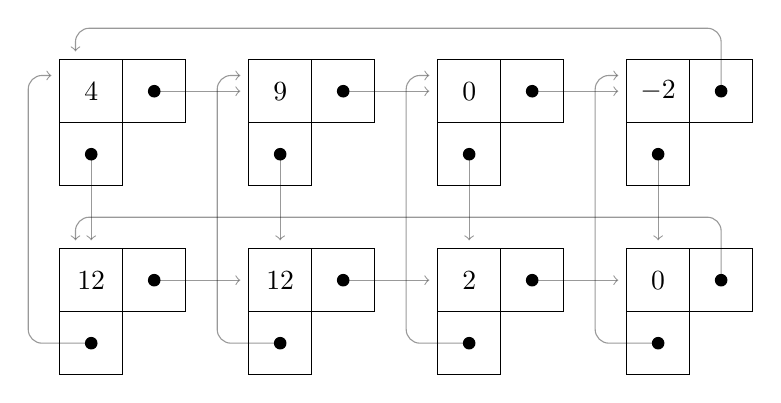
\begin{tikzpicture}[scale=.8,link/.style={opacity=.4,->,shorten >=3pt}]
\foreach \x in {0,1,2,3}{
  \foreach \y in {0,-1}{
    \draw (\x*3,\y*3) rectangle (\x*3+2,\y*3+1);
    \draw (\x*3,\y*3+1) rectangle (\x*3+1,\y*3-1);
  }
}
\foreach \x\y\n in {0/0/4, 1/0/9, 2/0/0, 3/0/-2, 0/-1/12, 1/-1/12, 2/-1/2, 3/-1/0 }{
  \node at (3*\x+.5,\y*3+.5) {$\n$};
  \fill[black] (3*\x+1.5,\y*3+.5) circle (.1);
  \fill[black] (3*\x+.5,\y*3-.5) circle (.1);
}
\foreach \x in {0,1,2}{
  \draw[link] (\x*3+1.5,.5)--(\x*3+3,.5);
  \draw[link] (\x*3+1.5,-2.5)--(\x*3+3,-2.5);
}
\foreach \x in {0,1,2,3}{
  \draw[link] (\x*3+.5,-.5)--(\x*3+.5,-2);
  \draw[link,rounded corners=5pt] (\x*3+.5,-3.5)--++(180:1)--++(90:4.25)--++(0:.5);
}

\draw[link,rounded corners=5pt] (10.5,.5)--++(90:1)--++(180:10.25)--++(270:.5);
\draw[link,rounded corners=5pt] (10.5,-2.5)--++(90:1)--++(180:10.25)--++(270:.5);
\end{tikzpicture}
\]




